\documentclass[11pt, a4paper]{article} % setsfont size and layout

%% required packages %%

\usepackage[margin=2.5cm]{geometry} % margins
\usepackage[utf8]{inputenc} % Umlaute
\usepackage{amsmath,amssymb}		% math formulas
\usepackage{graphicx}		% graphics
\usepackage{fancyhdr}		% header and footer on every page
\usepackage{setspace}		% line space (e.g. \singlespacing, \onehalfspacing or \doublespacing)

\usepackage{braket}
\usepackage{xcolor}
%% Here the main part of the document begins %%

\begin{document}
	
%% Some more settings %%
	
\setlength{\parindent}{0pt} % first line in paragraph will not be indented
\onehalfspacing				% 1.5 line spacing
%\thispagestyle{empty}		% no header and page number on first page


%% Header on first page with course information etc. %%
\begin{tabular}{p{15.5cm}}
	{\large \textbf{Classical Mechanics}} \\
	Westlake University \\ 
	\hline
	\\
\end{tabular}

\vspace*{0.1cm}				% vertical space between header on top of the page and main heading


%\begin{center}
%	{\Large \textbf{Final Exam}}
%	\vspace{2mm}
%Name: 
%\end{center} 
%\vspace{0.1cm}
{\bf \color{red} Deadline: 9:00 pm, Oct. 15th, 2025} \\
{\color{blue} All problem sets and your solutions must be kept private. Please do not share them publicly or with future students. All answers must be \textbf{handwritten}, then scanned or photographed, and submitted via Canvas. } 

\section*{Fermat's principle [25 points]} 
One of the most foundational principles in optics known as Fermat's principle, which states: ``\textit{The path taken by a light ray between any two points is the path that minimizes the travel time between the points}."

(a) Derive an expression for the total travel time of a light ray moving from point $a$ to point $b$, $T=\int_a^bdt$. Then, apply Fermat's Principle and use the calculus of variations to derive Snell's Law: $\frac{\sin \theta_1}{\sin \theta_2}=\frac{n_2}{n_1}$. [10 points]

(b) Suppose the refractive index of a material varies with vertical position $y$ as $n(y) = L/y$, where $L$ is a constant. Using Fermat's Principle, derive the path that a light ray takes when traveling from point $a$ to point $b$. [15 points]

\begin{figure}[h]
    \centering
    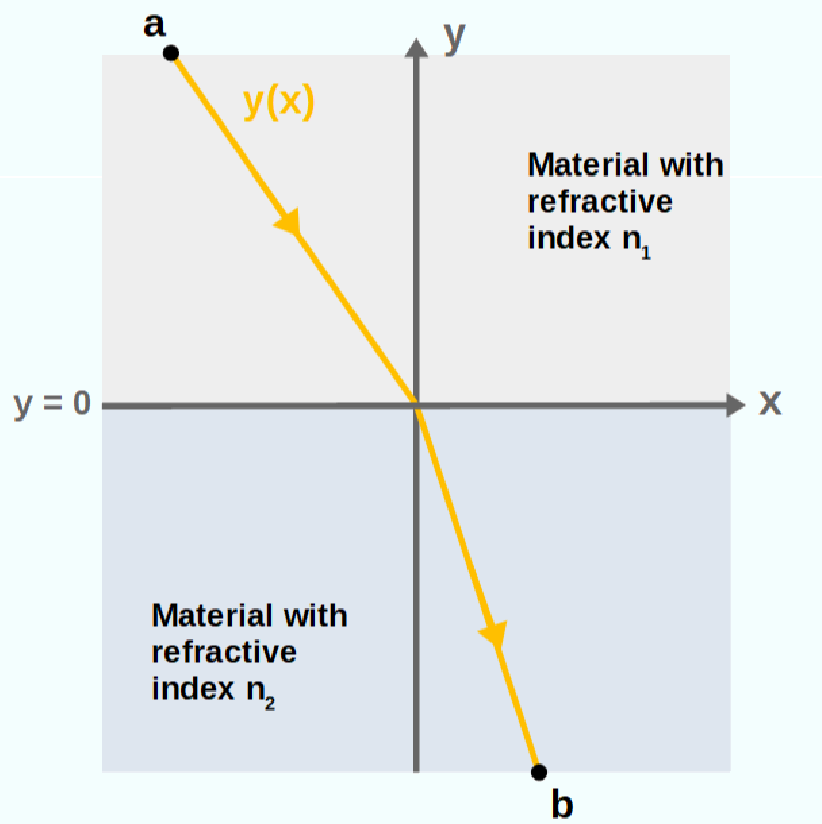
\includegraphics[width=0.5\textwidth]{Optics.png}
    \label{P2}
\end{figure}

\newpage
\section*{Spherical pendulum [15 points]} 
A ball of mass $m$ swings on the end of an unstretchable string of length $R$ in the presence of a uniform gravitational field $g$. This is often called the ``spherical pendulum,” because the ball moves as though it were sliding on the frictionless surface of a spherical bowl. It is important to note that:
(i) It can move horizontally around a vertical axis passing through the point of support, corresponding to changes in its azimuthal angle $\phi$. (On earth’s surface this would correspond to a change in longitude.) (ii) It can also move in the polar direction, as described by the angle $\theta$. (On earth’s surface this would correspond to a change in latitude.)
Please find its equations of motion (a second-order differential equation for the polar angle $\theta$ as a function of time). You do not need to solve the equation of motion.


\begin{figure}[h]
    \centering
    \includegraphics[width=0.4\textwidth]{PS2_P1.png}
    \label{P1}
%    \caption{Coordinates of a ball hanging on an unstretchable string.}
\end{figure}

\newpage
\section*{Pendulum with a spring [20 points]} 
A plane pendulum is made with a bob of mass $m$ hanging on a Hooke’s-law spring of negligible mass, force constant $k$, and unstretched length $l_0$. The spring can stretch but is not allowed to bend. There is a uniform downward gravitational field $g$. 

(a) Select generalized coordinates for the bob, and find the Lagrangian in terms of them. [4 points]

(b) Write out the Lagrange equations of motion. [4 points]

(c) Are there any conserved quantities? If so, write down the corresponding conservation law(s). [4 points]

(d) If the bob is swinging back and forth, find the frequency of small oscillations in the general case where the spring can change its length while the bob is swinging back and forth. [8 points]

\begin{figure}[h]
    \centering
    \includegraphics[width=0.5\textwidth]{PS2_P2.png}
    \label{P2}
\end{figure}

\newpage 
\section*{Non-uniqueness of Lagrangian [20 points]} 
Consider a Lagrangian $L'=L+df/dt$, where the Lagrangian is $L = L(q_k,\dot{q}_k,t)$ and the function $f=f(q_k,t)$. 

(a) Show that $L' = L'(q_k,\dot{q}_k,t)$, that is, $L'$ also depends on $q_k$, $\dot{q}_k$, and $t$. Show that this would not generally be true if $f$ were allowed to depend upon the $\dot{q}_k$. [8 points]

(b) Show that $L'$ obeys Euler-Lagrange equations if $L$ does, by substituting $L'$ into Euler-Lagrange equations. Therefore, the equations of motion are the same using $L'$ as using $L'$, so the Lagrangian of a particle is not unique. [12 points]

\newpage 
\section*{Problems from Classical Mechanics of John R. Taylor [104 points]} 
Chapter 7: 7.1, 7.3, 7.11 [$4\times3$ points]\\
Chapter 7: 7.13, 7.23, 7.29, 7.31 [$8\times4$ points]\\
Chapter 7: 7.43, 7.44. These two problems require coding. Please prepare your solutions as a Jupyter notebook and submit it to Westlake HPC Elastic Container Service.   [$30\times2$ points]\\
Bonus problem: We studied the brachistochrone problem in class. Please prepare a Jupyter notebook that includes a detailed derivation of the solution and a corresponding plot. [$25$ points]\\

\end{document}